\clearpage

{\chaptoc
  \section*{Compute Accounting}\addcontentsline{toc}{section}{Compute Accounting}
}


\subsection{Tensors On Gpus}~{}


\textbf{默认情况下},PyTorch 创建的张量会存储在 CPU 内存中:

为了利用 GPU 的大规模并行计算能力,需要将张量移动到 GPU 内存。

\begin{lstlisting}[language=Python]
# 默认创建在 CPU
x = torch.zeros(32, 32)
assert x.device == torch.device("cpu")

if torch.cuda.is_available():
    # GPU 属性
    for i in range(torch.cuda.device_count()):
        print(torch.cuda.get_device_properties(i))

    mem0 = torch.cuda.memory_allocated()

    # CPU -> GPU0
    y = x.to("cuda:0")
    assert y.device == torch.device("cuda", 0)

    # 或者直接在 GPU 创建
    z = torch.zeros(32, 32, device="cuda:0")
\end{lstlisting}

\begin{figure}[htbp]
  \centering
  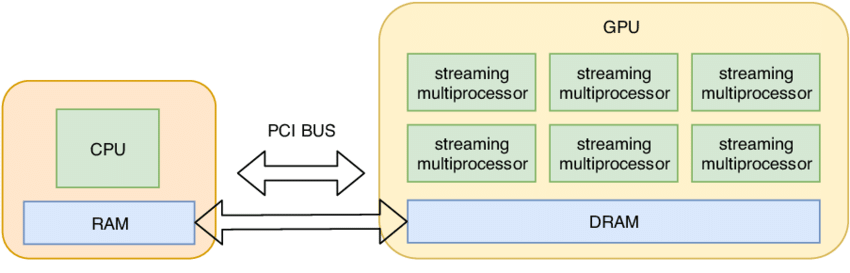
\includegraphics[width=0.9\linewidth]{figs/lec2/lec2.40.png}
  \caption{Move tensor from CPU to GPUs}
\end{figure}

heelp
\par
% \begin{itemize}
%     \item GPU 内存有限,通常只有几 GB
%     \item GPU 内存分配和释放开销较大
%     \item GPU 计算需要数据传输,传输开销较大    
% \end{itemize}




\subsection{Tensor Operations}
\subsection{Tensor Einops}
\subsection{Tensor Operations Flops}
\subsection{Gradients Basics}
\subsection{Gradients Flops}


\clearpage
{\chaptoc\noindent\begin{minipage}[inner sep=0,outer sep=0]{0.9\linewidth}\section{Models}
\end{minipage}}
\subsection{Module Parameters}
\subsection{Custom Model}



\clearpage
{\chaptoc\noindent\begin{minipage}[inner sep=0,outer sep=0]{0.9\linewidth}\section{Training Loop And Best Practices}
\end{minipage}}
\subsection{Note About Randomness}
\subsection{Data Loading}
\subsection{Optimizer}
\subsection{Train Loop}
\subsection{Checkpointing}

\clearpage
